\documentclass{article}
\usepackage[utf8]{inputenc}
\usepackage[T2A]{fontenc}
\usepackage[russian]{babel}
\usepackage{graphicx} % Для вставки изображений

\title{Пример документа с таблицей и каким-то пеликаном}
\author{Анастасия Шпилева}
\date{\today}

\begin{document}

\maketitle

\begin{figure}[htbp]
\centering
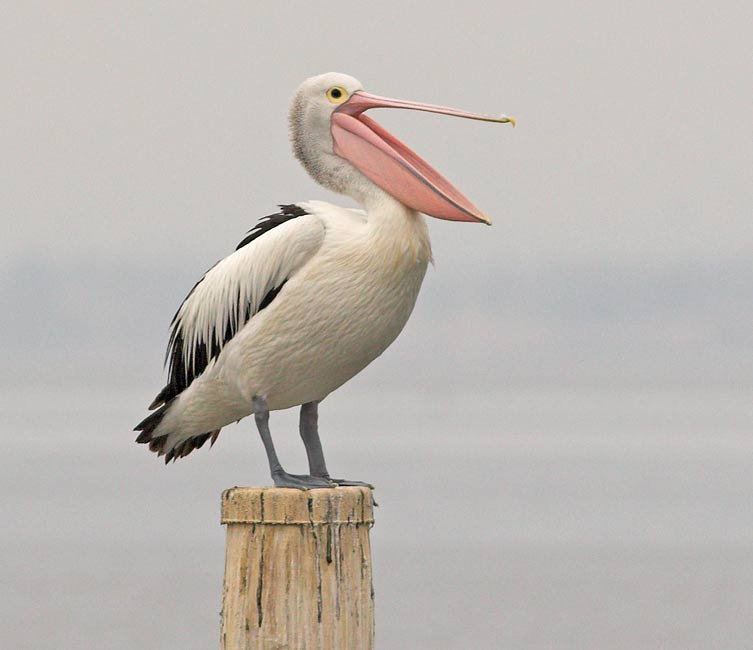
\includegraphics[width=0.5\textwidth]{artifacts/image.jpg}
\caption{Пеликан (жестко удивляется)}
\label{fig:example}
\end{figure}

\begin{table}[htbp]
\centering
\caption{Пример таблицы с каким-то 
 содержимом и пеликаном}
\label{tab:pelicans}
\begin{tabular}{|cccc|}
\hline
Столбец 1 & Столбец 2 & Столбец 3 & Столбец 4 \\
1 & 10 & 2.5 & Mister \\
2 & 5 & 3.2 & pelican \\
3 & 8 & 4.1 & is \\
4 & 12 & 3.8 & standing \\
\hline
\end{tabular}
\end{table}

\end{document}
